\documentclass[../_main/handlingar.tex]{subfiles}

\begin{document}
\motion{Att-satsernas fortlevnad}

Det är för lite att-satser nuförtiden.

\begin{center}
    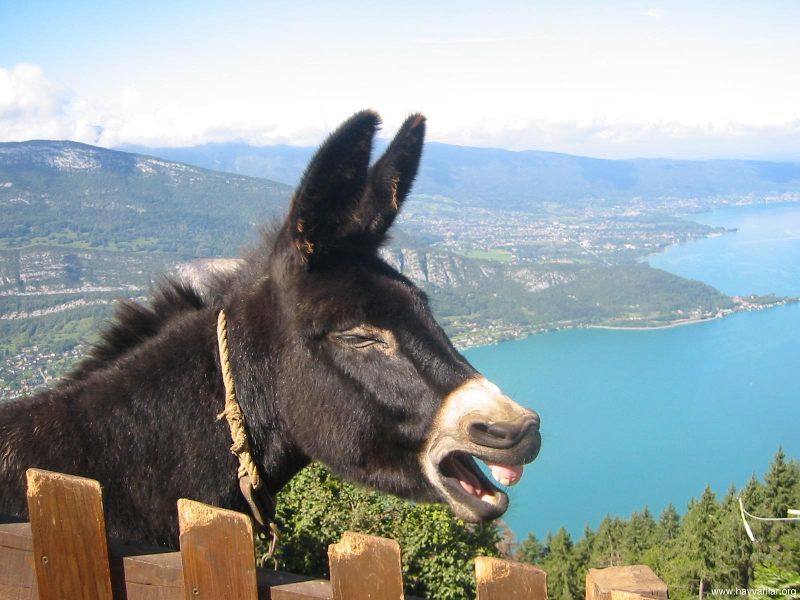
\includegraphics[width=10cm]{esek.jpg}
\end{center}

Därför yrkar vi på
\begin{attsatser}
    \att skriva fler att-satser.
    \att
    skriva att-satser\\
    som sträcker\\
    sig över\\
    flera rader.
    \att under \S0 i stadgarna lägga till\par
    \begin{itshape}
        ``att'':
        \begin{itemizedash}
            \item att
            \item \sout{att}
            \item \hl{att}
        \end{itemizedash}
    \end{itshape}
\end{attsatser}

\begin{signatures}{2}
    \mvh
    \signature{Erik Månsson}{Kontaktor}
    \signature{Måns Eriksson}{Någon som håller med}
\end{signatures}

\end{document}
